% Created by tikzDevice version 0.7.0 on 2014-10-06 20:10:14
% !TEX encoding = UTF-8 Unicode
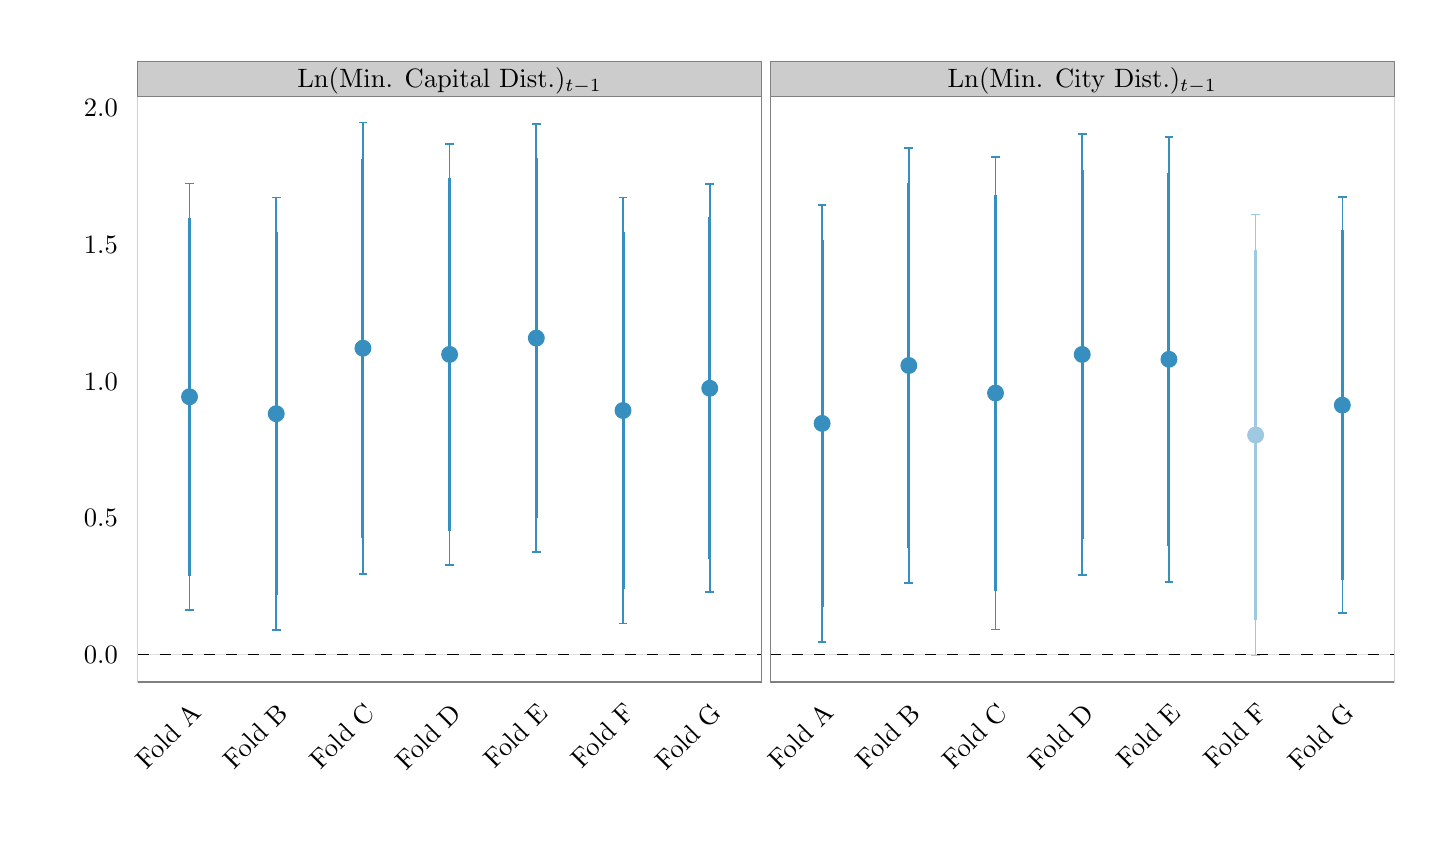
\begin{tikzpicture}[x=1pt,y=1pt]
\definecolor[named]{fillColor}{rgb}{1.00,1.00,1.00}
\path[use as bounding box,fill=fillColor,fill opacity=0.00] (0,0) rectangle (505.89,289.08);
\begin{scope}
\path[clip] (  0.00,  0.00) rectangle (505.89,289.08);
\definecolor[named]{drawColor}{rgb}{1.00,1.00,1.00}
\definecolor[named]{fillColor}{rgb}{1.00,1.00,1.00}

\path[draw=drawColor,line width= 0.6pt,line join=round,line cap=round,fill=fillColor] (  0.00,  0.00) rectangle (505.89,289.08);
\end{scope}
\begin{scope}
\path[clip] ( 39.69, 52.60) rectangle (265.26,264.40);
\definecolor[named]{fillColor}{rgb}{1.00,1.00,1.00}

\path[fill=fillColor] ( 39.69, 52.60) rectangle (265.26,264.40);
\definecolor[named]{drawColor}{rgb}{0.21,0.56,0.75}
\definecolor[named]{fillColor}{rgb}{0.21,0.56,0.75}

\path[draw=drawColor,draw opacity=0.30,line width= 0.3pt,line join=round,fill=fillColor,fill opacity=0.30] ( 58.48, 78.70) -- ( 58.48,232.72);

\path[draw=drawColor,draw opacity=0.30,line width= 0.3pt,line join=round,fill=fillColor,fill opacity=0.30] ( 89.81, 71.45) -- ( 89.81,227.72);

\path[draw=drawColor,draw opacity=0.30,line width= 0.3pt,line join=round,fill=fillColor,fill opacity=0.30] (121.14, 91.74) -- (121.14,254.77);

\path[draw=drawColor,draw opacity=0.30,line width= 0.3pt,line join=round,fill=fillColor,fill opacity=0.30] (152.47, 95.01) -- (152.47,247.01);

\path[draw=drawColor,draw opacity=0.30,line width= 0.3pt,line join=round,fill=fillColor,fill opacity=0.30] (183.80, 99.56) -- (183.80,254.25);

\path[draw=drawColor,draw opacity=0.30,line width= 0.3pt,line join=round,fill=fillColor,fill opacity=0.30] (215.13, 73.72) -- (215.13,227.75);

\path[draw=drawColor,draw opacity=0.30,line width= 0.3pt,line join=round,fill=fillColor,fill opacity=0.30] (246.46, 85.07) -- (246.46,232.49);
\definecolor[named]{drawColor}{rgb}{0.21,0.56,0.75}
\definecolor[named]{fillColor}{rgb}{0.21,0.56,0.75}

\path[draw=drawColor,line width= 1.1pt,line join=round,fill=fillColor] ( 58.48, 91.09) -- ( 58.48,220.34);

\path[draw=drawColor,line width= 1.1pt,line join=round,fill=fillColor] ( 89.81, 84.01) -- ( 89.81,215.15);

\path[draw=drawColor,line width= 1.1pt,line join=round,fill=fillColor] (121.14,104.85) -- (121.14,241.67);

\path[draw=drawColor,line width= 1.1pt,line join=round,fill=fillColor] (152.47,107.23) -- (152.47,234.79);

\path[draw=drawColor,line width= 1.1pt,line join=round,fill=fillColor] (183.80,111.99) -- (183.80,241.82);

\path[draw=drawColor,line width= 1.1pt,line join=round,fill=fillColor] (215.13, 86.11) -- (215.13,215.37);

\path[draw=drawColor,line width= 1.1pt,line join=round,fill=fillColor] (246.46, 96.92) -- (246.46,220.64);
\definecolor[named]{drawColor}{rgb}{0.00,0.00,0.00}
\definecolor[named]{fillColor}{rgb}{0.00,0.00,0.00}

\path[draw=drawColor,line width= 0.6pt,dash pattern=on 4pt off 4pt ,line join=round,fill=fillColor] ( 39.69, 62.52) -- (265.26, 62.52);
\definecolor[named]{drawColor}{rgb}{0.21,0.56,0.75}
\definecolor[named]{fillColor}{rgb}{0.21,0.56,0.75}

\path[draw=drawColor,line width= 0.4pt,line join=round,line cap=round,fill=fillColor] ( 58.48,155.71) circle (  2.85);

\path[draw=drawColor,line width= 0.4pt,line join=round,line cap=round,fill=fillColor] ( 89.81,149.58) circle (  2.85);

\path[draw=drawColor,line width= 0.4pt,line join=round,line cap=round,fill=fillColor] (121.14,173.26) circle (  2.85);

\path[draw=drawColor,line width= 0.4pt,line join=round,line cap=round,fill=fillColor] (152.47,171.01) circle (  2.85);

\path[draw=drawColor,line width= 0.4pt,line join=round,line cap=round,fill=fillColor] (183.80,176.91) circle (  2.85);

\path[draw=drawColor,line width= 0.4pt,line join=round,line cap=round,fill=fillColor] (215.13,150.74) circle (  2.85);

\path[draw=drawColor,line width= 0.4pt,line join=round,line cap=round,fill=fillColor] (246.46,158.78) circle (  2.85);

\path[draw=drawColor,line width= 0.6pt,line join=round] ( 56.92,232.72) --
	( 60.05,232.72);

\path[draw=drawColor,line width= 0.6pt,line join=round] ( 58.48,232.72) --
	( 58.48, 78.70);

\path[draw=drawColor,line width= 0.6pt,line join=round] ( 56.92, 78.70) --
	( 60.05, 78.70);

\path[draw=drawColor,line width= 0.6pt,line join=round] ( 88.25,227.72) --
	( 91.38,227.72);

\path[draw=drawColor,line width= 0.6pt,line join=round] ( 89.81,227.72) --
	( 89.81, 71.45);

\path[draw=drawColor,line width= 0.6pt,line join=round] ( 88.25, 71.45) --
	( 91.38, 71.45);

\path[draw=drawColor,line width= 0.6pt,line join=round] (119.58,254.77) --
	(122.71,254.77);

\path[draw=drawColor,line width= 0.6pt,line join=round] (121.14,254.77) --
	(121.14, 91.74);

\path[draw=drawColor,line width= 0.6pt,line join=round] (119.58, 91.74) --
	(122.71, 91.74);

\path[draw=drawColor,line width= 0.6pt,line join=round] (150.91,247.01) --
	(154.04,247.01);

\path[draw=drawColor,line width= 0.6pt,line join=round] (152.47,247.01) --
	(152.47, 95.01);

\path[draw=drawColor,line width= 0.6pt,line join=round] (150.91, 95.01) --
	(154.04, 95.01);

\path[draw=drawColor,line width= 0.6pt,line join=round] (182.24,254.25) --
	(185.37,254.25);

\path[draw=drawColor,line width= 0.6pt,line join=round] (183.80,254.25) --
	(183.80, 99.56);

\path[draw=drawColor,line width= 0.6pt,line join=round] (182.24, 99.56) --
	(185.37, 99.56);

\path[draw=drawColor,line width= 0.6pt,line join=round] (213.57,227.75) --
	(216.70,227.75);

\path[draw=drawColor,line width= 0.6pt,line join=round] (215.13,227.75) --
	(215.13, 73.72);

\path[draw=drawColor,line width= 0.6pt,line join=round] (213.57, 73.72) --
	(216.70, 73.72);

\path[draw=drawColor,line width= 0.6pt,line join=round] (244.90,232.49) --
	(248.03,232.49);

\path[draw=drawColor,line width= 0.6pt,line join=round] (246.46,232.49) --
	(246.46, 85.07);

\path[draw=drawColor,line width= 0.6pt,line join=round] (244.90, 85.07) --
	(248.03, 85.07);
\definecolor[named]{drawColor}{rgb}{0.50,0.50,0.50}

\path[draw=drawColor,line width= 0.6pt,line join=round,line cap=round] ( 39.69, 52.60) rectangle (265.26,264.40);
\end{scope}
\begin{scope}
\path[clip] (268.27, 52.60) rectangle (493.85,264.40);
\definecolor[named]{fillColor}{rgb}{1.00,1.00,1.00}

\path[fill=fillColor] (268.27, 52.60) rectangle (493.85,264.40);
\definecolor[named]{drawColor}{rgb}{0.21,0.56,0.75}
\definecolor[named]{fillColor}{rgb}{0.21,0.56,0.75}

\path[draw=drawColor,draw opacity=0.30,line width= 0.3pt,line join=round,fill=fillColor,fill opacity=0.30] (287.07, 67.19) -- (287.07,224.97);

\path[draw=drawColor,draw opacity=0.30,line width= 0.3pt,line join=round,fill=fillColor,fill opacity=0.30] (318.40, 88.38) -- (318.40,245.63);

\path[draw=drawColor,draw opacity=0.30,line width= 0.3pt,line join=round,fill=fillColor,fill opacity=0.30] (349.73, 71.61) -- (349.73,242.46);

\path[draw=drawColor,draw opacity=0.30,line width= 0.3pt,line join=round,fill=fillColor,fill opacity=0.30] (381.06, 91.40) -- (381.06,250.60);

\path[draw=drawColor,draw opacity=0.30,line width= 0.3pt,line join=round,fill=fillColor,fill opacity=0.30] (412.39, 88.88) -- (412.39,249.59);
\definecolor[named]{drawColor}{rgb}{0.62,0.79,0.88}
\definecolor[named]{fillColor}{rgb}{0.62,0.79,0.88}

\path[draw=drawColor,draw opacity=0.30,line width= 0.3pt,line join=round,fill=fillColor,fill opacity=0.30] (443.72, 62.23) -- (443.72,221.53);
\definecolor[named]{drawColor}{rgb}{0.21,0.56,0.75}
\definecolor[named]{fillColor}{rgb}{0.21,0.56,0.75}

\path[draw=drawColor,draw opacity=0.30,line width= 0.3pt,line join=round,fill=fillColor,fill opacity=0.30] (475.05, 77.47) -- (475.05,227.88);
\definecolor[named]{drawColor}{rgb}{0.21,0.56,0.75}
\definecolor[named]{fillColor}{rgb}{0.21,0.56,0.75}

\path[draw=drawColor,line width= 1.1pt,line join=round,fill=fillColor] (287.07, 79.88) -- (287.07,212.29);

\path[draw=drawColor,line width= 1.1pt,line join=round,fill=fillColor] (318.40,101.02) -- (318.40,232.99);

\path[draw=drawColor,line width= 1.1pt,line join=round,fill=fillColor] (349.73, 85.35) -- (349.73,228.72);

\path[draw=drawColor,line width= 1.1pt,line join=round,fill=fillColor] (381.06,104.20) -- (381.06,237.81);

\path[draw=drawColor,line width= 1.1pt,line join=round,fill=fillColor] (412.39,101.80) -- (412.39,236.67);
\definecolor[named]{drawColor}{rgb}{0.62,0.79,0.88}
\definecolor[named]{fillColor}{rgb}{0.62,0.79,0.88}

\path[draw=drawColor,line width= 1.1pt,line join=round,fill=fillColor] (443.72, 75.03) -- (443.72,208.73);
\definecolor[named]{drawColor}{rgb}{0.21,0.56,0.75}
\definecolor[named]{fillColor}{rgb}{0.21,0.56,0.75}

\path[draw=drawColor,line width= 1.1pt,line join=round,fill=fillColor] (475.05, 89.56) -- (475.05,215.79);
\definecolor[named]{drawColor}{rgb}{0.00,0.00,0.00}
\definecolor[named]{fillColor}{rgb}{0.00,0.00,0.00}

\path[draw=drawColor,line width= 0.6pt,dash pattern=on 4pt off 4pt ,line join=round,fill=fillColor] (268.27, 62.52) -- (493.85, 62.52);
\definecolor[named]{drawColor}{rgb}{0.21,0.56,0.75}
\definecolor[named]{fillColor}{rgb}{0.21,0.56,0.75}

\path[draw=drawColor,line width= 0.4pt,line join=round,line cap=round,fill=fillColor] (287.07,146.08) circle (  2.85);

\path[draw=drawColor,line width= 0.4pt,line join=round,line cap=round,fill=fillColor] (318.40,167.00) circle (  2.85);

\path[draw=drawColor,line width= 0.4pt,line join=round,line cap=round,fill=fillColor] (349.73,157.04) circle (  2.85);

\path[draw=drawColor,line width= 0.4pt,line join=round,line cap=round,fill=fillColor] (381.06,171.00) circle (  2.85);

\path[draw=drawColor,line width= 0.4pt,line join=round,line cap=round,fill=fillColor] (412.39,169.24) circle (  2.85);
\definecolor[named]{drawColor}{rgb}{0.62,0.79,0.88}
\definecolor[named]{fillColor}{rgb}{0.62,0.79,0.88}

\path[draw=drawColor,line width= 0.4pt,line join=round,line cap=round,fill=fillColor] (443.72,141.88) circle (  2.85);
\definecolor[named]{drawColor}{rgb}{0.21,0.56,0.75}
\definecolor[named]{fillColor}{rgb}{0.21,0.56,0.75}

\path[draw=drawColor,line width= 0.4pt,line join=round,line cap=round,fill=fillColor] (475.05,152.67) circle (  2.85);

\path[draw=drawColor,line width= 0.6pt,line join=round] (285.50,224.97) --
	(288.64,224.97);

\path[draw=drawColor,line width= 0.6pt,line join=round] (287.07,224.97) --
	(287.07, 67.19);

\path[draw=drawColor,line width= 0.6pt,line join=round] (285.50, 67.19) --
	(288.64, 67.19);

\path[draw=drawColor,line width= 0.6pt,line join=round] (316.83,245.63) --
	(319.97,245.63);

\path[draw=drawColor,line width= 0.6pt,line join=round] (318.40,245.63) --
	(318.40, 88.38);

\path[draw=drawColor,line width= 0.6pt,line join=round] (316.83, 88.38) --
	(319.97, 88.38);

\path[draw=drawColor,line width= 0.6pt,line join=round] (348.16,242.46) --
	(351.30,242.46);

\path[draw=drawColor,line width= 0.6pt,line join=round] (349.73,242.46) --
	(349.73, 71.61);

\path[draw=drawColor,line width= 0.6pt,line join=round] (348.16, 71.61) --
	(351.30, 71.61);

\path[draw=drawColor,line width= 0.6pt,line join=round] (379.49,250.60) --
	(382.62,250.60);

\path[draw=drawColor,line width= 0.6pt,line join=round] (381.06,250.60) --
	(381.06, 91.40);

\path[draw=drawColor,line width= 0.6pt,line join=round] (379.49, 91.40) --
	(382.62, 91.40);

\path[draw=drawColor,line width= 0.6pt,line join=round] (410.82,249.59) --
	(413.95,249.59);

\path[draw=drawColor,line width= 0.6pt,line join=round] (412.39,249.59) --
	(412.39, 88.88);

\path[draw=drawColor,line width= 0.6pt,line join=round] (410.82, 88.88) --
	(413.95, 88.88);
\definecolor[named]{drawColor}{rgb}{0.62,0.79,0.88}

\path[draw=drawColor,line width= 0.6pt,line join=round] (442.15,221.53) --
	(445.28,221.53);

\path[draw=drawColor,line width= 0.6pt,line join=round] (443.72,221.53) --
	(443.72, 62.23);

\path[draw=drawColor,line width= 0.6pt,line join=round] (442.15, 62.23) --
	(445.28, 62.23);
\definecolor[named]{drawColor}{rgb}{0.21,0.56,0.75}

\path[draw=drawColor,line width= 0.6pt,line join=round] (473.48,227.88) --
	(476.61,227.88);

\path[draw=drawColor,line width= 0.6pt,line join=round] (475.05,227.88) --
	(475.05, 77.47);

\path[draw=drawColor,line width= 0.6pt,line join=round] (473.48, 77.47) --
	(476.61, 77.47);
\definecolor[named]{drawColor}{rgb}{0.50,0.50,0.50}

\path[draw=drawColor,line width= 0.6pt,line join=round,line cap=round] (268.27, 52.60) rectangle (493.85,264.40);
\end{scope}
\begin{scope}
\path[clip] (  0.00,  0.00) rectangle (505.89,289.08);
\definecolor[named]{drawColor}{rgb}{0.50,0.50,0.50}
\definecolor[named]{fillColor}{rgb}{0.80,0.80,0.80}

\path[draw=drawColor,line width= 0.2pt,line join=round,line cap=round,fill=fillColor] ( 39.69,264.40) rectangle (265.26,277.04);
\definecolor[named]{drawColor}{rgb}{0.00,0.00,0.00}

\node[text=drawColor,anchor=base,inner sep=0pt, outer sep=0pt, scale=  0.96] at (152.47,267.41) {Ln(Min. Capital Dist.)$_{t-1}$};
\end{scope}
\begin{scope}
\path[clip] (  0.00,  0.00) rectangle (505.89,289.08);
\definecolor[named]{drawColor}{rgb}{0.50,0.50,0.50}
\definecolor[named]{fillColor}{rgb}{0.80,0.80,0.80}

\path[draw=drawColor,line width= 0.2pt,line join=round,line cap=round,fill=fillColor] (268.27,264.40) rectangle (493.85,277.04);
\definecolor[named]{drawColor}{rgb}{0.00,0.00,0.00}

\node[text=drawColor,anchor=base,inner sep=0pt, outer sep=0pt, scale=  0.96] at (381.06,267.41) {Ln(Min. City Dist.)$_{t-1}$};
\end{scope}
\begin{scope}
\path[clip] (  0.00,  0.00) rectangle (505.89,289.08);
\definecolor[named]{drawColor}{rgb}{0.00,0.00,0.00}

\node[text=drawColor,anchor=base east,inner sep=0pt, outer sep=0pt, scale=  0.96] at ( 32.57, 59.21) {0.0};

\node[text=drawColor,anchor=base east,inner sep=0pt, outer sep=0pt, scale=  0.96] at ( 32.57,108.66) {0.5};

\node[text=drawColor,anchor=base east,inner sep=0pt, outer sep=0pt, scale=  0.96] at ( 32.57,158.12) {1.0};

\node[text=drawColor,anchor=base east,inner sep=0pt, outer sep=0pt, scale=  0.96] at ( 32.57,207.57) {1.5};

\node[text=drawColor,anchor=base east,inner sep=0pt, outer sep=0pt, scale=  0.96] at ( 32.57,257.02) {2.0};
\end{scope}
\begin{scope}
\path[clip] (  0.00,  0.00) rectangle (505.89,289.08);
\definecolor[named]{drawColor}{rgb}{0.00,0.00,0.00}

\node[text=drawColor,rotate= 45.00,anchor=base east,inner sep=0pt, outer sep=0pt, scale=  0.96] at ( 63.16, 40.81) {Fold A};

\node[text=drawColor,rotate= 45.00,anchor=base east,inner sep=0pt, outer sep=0pt, scale=  0.96] at ( 94.49, 40.81) {Fold B};

\node[text=drawColor,rotate= 45.00,anchor=base east,inner sep=0pt, outer sep=0pt, scale=  0.96] at (125.82, 40.81) {Fold C};

\node[text=drawColor,rotate= 45.00,anchor=base east,inner sep=0pt, outer sep=0pt, scale=  0.96] at (157.15, 40.81) {Fold D};

\node[text=drawColor,rotate= 45.00,anchor=base east,inner sep=0pt, outer sep=0pt, scale=  0.96] at (188.48, 40.81) {Fold E};

\node[text=drawColor,rotate= 45.00,anchor=base east,inner sep=0pt, outer sep=0pt, scale=  0.96] at (219.81, 40.81) {Fold F};

\node[text=drawColor,rotate= 45.00,anchor=base east,inner sep=0pt, outer sep=0pt, scale=  0.96] at (251.14, 40.81) {Fold G};
\end{scope}
\begin{scope}
\path[clip] (  0.00,  0.00) rectangle (505.89,289.08);
\definecolor[named]{drawColor}{rgb}{0.00,0.00,0.00}

\node[text=drawColor,rotate= 45.00,anchor=base east,inner sep=0pt, outer sep=0pt, scale=  0.96] at (291.74, 40.81) {Fold A};

\node[text=drawColor,rotate= 45.00,anchor=base east,inner sep=0pt, outer sep=0pt, scale=  0.96] at (323.07, 40.81) {Fold B};

\node[text=drawColor,rotate= 45.00,anchor=base east,inner sep=0pt, outer sep=0pt, scale=  0.96] at (354.40, 40.81) {Fold C};

\node[text=drawColor,rotate= 45.00,anchor=base east,inner sep=0pt, outer sep=0pt, scale=  0.96] at (385.73, 40.81) {Fold D};

\node[text=drawColor,rotate= 45.00,anchor=base east,inner sep=0pt, outer sep=0pt, scale=  0.96] at (417.06, 40.81) {Fold E};

\node[text=drawColor,rotate= 45.00,anchor=base east,inner sep=0pt, outer sep=0pt, scale=  0.96] at (448.39, 40.81) {Fold F};

\node[text=drawColor,rotate= 45.00,anchor=base east,inner sep=0pt, outer sep=0pt, scale=  0.96] at (479.72, 40.81) {Fold G};
\end{scope}
\end{tikzpicture}
